\chapter{Design and Implementation}
\label{cha:implementation}
implement canvas fingerprinting -> intresting and has many different aspects


* hashes are used to reduce the amount of data for fast and easy comparison (among other uses).
* small variations and differences in the input that are not noticeable to the human eye
* hashing functions are non-reversible

(\textcite{multilogin17})

* canvas fingerprinting starts when rendering canvas
* all fonts contain glyphs ->  set of paths or closed curves that are specified using a particular mathematical formula. 
* e.g. lower case “i” has two glyphs, one for the dot and one for the body
* These particular glyphs, which are also known as outlines, are then filled with pixels to create the final letter form.
(\textcite{multilogin17})

What makes each canvas fingerprint unique is not the final image that we see, but how each computer renders hinting and anti-aliasing.
* hinting: Hints are basically instructions that are executed when the glyphs are drawn on your screen. These instructions move some of the points which define the shape of the letters, in order to make sure they are positioned correctly in relation to the grid where the glyph is displayed. This way, the font will look the same regardless of what screen it’s displayed on.
* anti-alisaing: may be the most common filter used today, and it consists of using gray pixels to smudge the edges of each glyph. If you zoom into a page, you’ll notice that the edges of curved letters are not perfect, but are rather jagged. The anti-aliasing filter smoothes out these jagged edges because our eyes average out the difference in tonality.
(\textcite{multilogin17})

\section{Idea}

\section{Architecture}

\subsection{Application scenario}

This chapter discusses the techniques introduced in \autoref{sec:Techniques} in form of a small application scenario. It concludes with a comparison which mounts to the one technique which is used for the prototype in \hyperref[cha:implementation]{chapter 5}.

\begin{figure}[H]
	\centering
	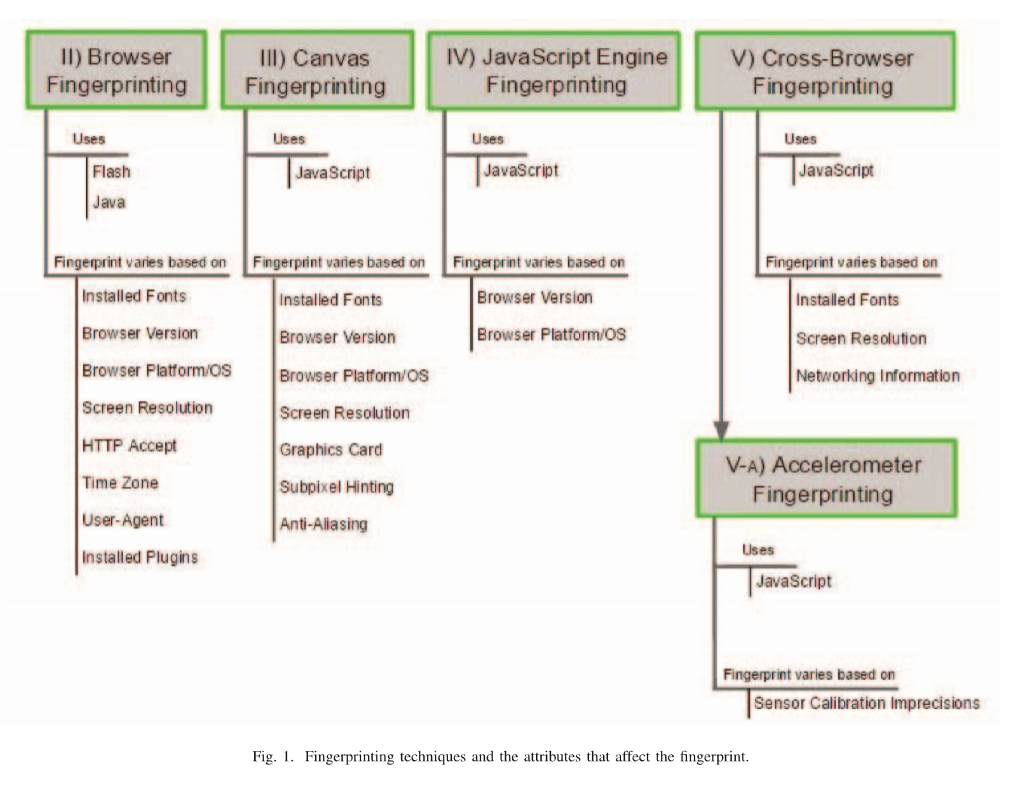
\includegraphics[width=350pt, height=160pt]{FingerprintingAttributes.png}
	\caption{Fingerprinting techniques and the attributes that effect the fingerprint}
	\label{BrowserSpecification}
\end{figure}

-- refere to previous chapter
-- give good overview what needs what?


\section{Programming}


\section{Obtained Data}


\section{Fingerprint}

\subsection{Calculation}

\section{Visualisation}